
\documentclass[12pt]{article}
\usepackage{graphicx}

\usepackage[a4paper,margin=2.5cm]{geometry}

\usepackage{amsmath,amsthm,amssymb}
\usepackage{thmtools}
\declaretheorem{theorem}
\usepackage{fancyhdr}
\pagestyle{fancy}
%\newtheorem{theorem}{Theorem}
\newtheorem{lemma}{Lemma}
\newtheorem{problem}{Problem}
\newtheorem{exercise}{Exercise}
\newtheorem{reflection}{Reflection}
\newtheorem{proposition}{Proposition}
\newtheorem{corollary}{Corollary}
\newtheorem{p}{Proof}
\newtheorem{axiom}{Axiom}


\newcommand{\N}{\mathbb{N}}
\newcommand{\Z}{\mathbb{Z}}
\newcommand{\R}{\mathbb{R}}
\newcommand{\Q}{\mathbb{Q}}
\newcommand{\C}{\mathbb{C}}
\newcommand{\I}{\mathbb{I}}

\lhead{Basic Mathematics, Serge Lange}
\chead{Joshua Jones}
\rhead{\today}
 
\begin{document}
\tableofcontents
\section{Available Elements}
These environments can be used to structure the document:
\begin{itemize}
	\item Axiom
	\item Proof
	\item Theorem
	\item Lemma
	\item Problem
	\item Exercise
	\item Reflection
	\item Proposition
	\item Corollary
\end{itemize}


\section{Examples}

\begin{axiom}[0 added to any natural number returns the same  ]
	\begin{equation}
		a+0=a
	\end{equation}		
\end{axiom}

\begin{axiom}[Successor Function]
The successor function is part of the formal language used to state the Peano axioms, which formalise the structure of the natural numbers.

\begin{equation}
S(n) = n+1
\end{equation}
\end{axiom}

\begin{p}[Proof title]
	\begin{proof}[Proof Title]
		This is a proof.
	\end{proof}
\end{p}

\begin{proof}[Proof Title]
	This is a proof.
\end{proof}

\begin{theorem}[Theorem Title]
	This is a theorem.
\end{theorem}

\begin{theorem}[Theorem Title]
	This is a theorem.
\end{theorem}

\begin{lemma}[Lemma Title]
	This is a lemma.
\end{lemma}

\begin{problem}[Problem Title]
This is a problem.
\end{problem}

\begin{exercise}[Exercise Title]
	This is an exercise.
\end{exercise}

\begin{reflection}[Reflection Title]
	This is a reflection.
\end{reflection}

\begin{proposition}[Proposition Title]
	This is a proposition.
\end{proposition}

\begin{corollary}[Corollary Title]
	This is a corollary.
\end{corollary}

\newpage
\section{Symbols to Identify Sets}
\begin{equation}
	\begin{split}
		\emptyset \text{ The empty set } \{ \}\\
		\N \text{ The set of Natural Numbers } \{0,1,2,3, ...\}\\
		\Z \text{ The set of Integers } \{...,-2,-1,0,1,2,...\}\\
		\Q \text{ The set of Rational Numbers}\\
		\I \text{ The set of Irrational Numbers}\\
		\R \text{ The set of Real Numbers}\\
		\C \text{ The set of Complex Numbers}
	\end{split}
\end{equation}

\begin{equation}
	\N \subset \Z \subset \Q \subset \R \subset \C
\end{equation}


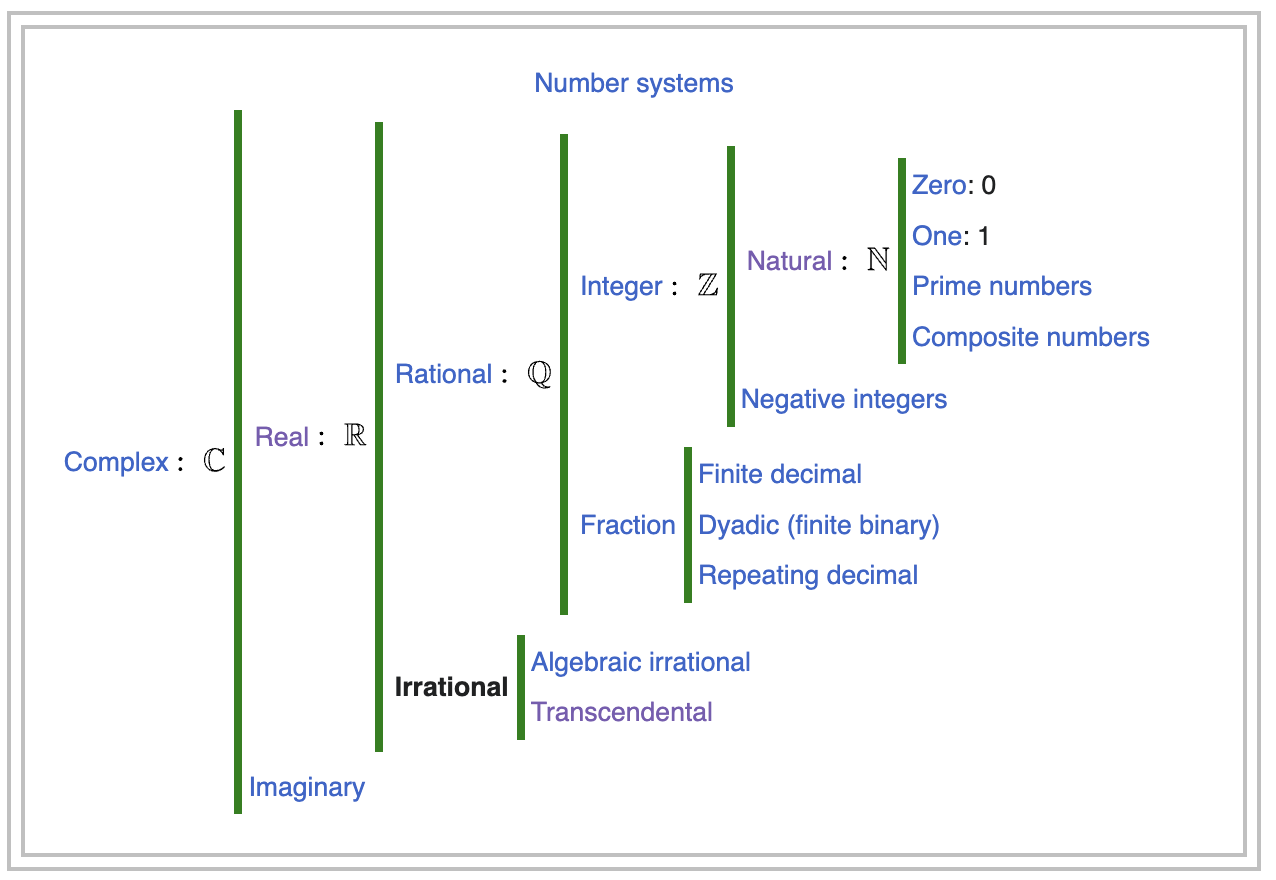
\includegraphics[width=\textwidth]{number_system.png}

\listoftheorems
\end{document}